%! TeX root = ../../main-en.tex
% 译自: backmatter/zh/appendix.tex @ 9048155:backmatter/zh/appendix.tex
\chapter{A Short History of Operating Systems}
\label{app:os-history}

Most of today's computers and phones run one of four operating systems: Windows, Linux, macOS or Android. All of them are ``modern operating systems'': they can run many programs at the same time, they use virtual memory to keep programs apart (Chapter~\ref{chap:memory}), and they serve programs through system calls (Chapter~\ref{chap:os}). Seen from the kernel, they all do much the same job.

Yet they feel very different to use. This appendix first tells you where they came from, and then explains why they feel so different. You don't need any of it to read this book; truly understanding how an operating system works often takes years. For now, ``oh, so that's how it is'' is all you need.

\section{A Family Tree}

The history of operating systems looks like a big, bushy family tree (Figure~\ref{fig:os-tree}). Today's four ``cousins'' come from just two ancestors: \emph{Unix}, born at Bell Labs in 1969, and \emph{DOS}, which arrived with the IBM PC in 1981.

\begin{figure}[htbp]
  \centering
  \begin{tikzpicture}[
      os/.style={draw, rounded corners=3pt, font=\small, minimum height=6mm, inner sep=3pt, align=center},
      unix/.style={os, fill=green!15},
      ms/.style={os, fill=blue!12},
      apple/.style={os, fill=gray!15},
      link/.style={-{Stealth}, thick, gray!70!black},
      idea/.style={-{Stealth}, dashed, gray},
      yr/.style={font=\scriptsize, gray!70!black, anchor=east},
      line width=0.6pt,
    ]
    % Years
    \foreach \y/\t in {0/1969, -1.3/1980s, -2.6/1990s, -3.9/2000s, -5.2/Today}
      \node[yr] at (-0.4,\y) {\t};
    \draw[gray!40] (-0.3,0.3) -- (-0.3,-5.5);

    % The Unix branch
    \node[unix] (unix)  at (2.4,0)    {Unix\\\scriptsize Bell Labs};
    \node[unix] (bsd)   at (1.2,-1.3) {BSD\\\scriptsize Berkeley};
    \node[unix] (minix) at (3.6,-1.3) {Minix\\\scriptsize for teaching};
    \node[unix] (linux) at (3.6,-2.6) {Linux\\\scriptsize 1991};
    \node[apple](next)  at (1.2,-2.6) {NeXTSTEP};
    \node[apple](mac)   at (1.2,-3.9) {Mac OS X\\\scriptsize 2001};
    \node[apple](macos) at (0.4,-5.2) {macOS};
    \node[apple](ios)   at (1.5,-5.2) {iOS};
    \node[unix] (distro)at (3.0,-5.2) {Ubuntu etc.\\\scriptsize distros};
    \node[unix] (andr)  at (5.0,-5.2) {Android\\\scriptsize 2008};

    \draw[link] (unix) -- (bsd);
    \draw[idea] (unix) -- (minix);
    \draw[idea] (minix) -- node[right, pos=0.4, font=\scriptsize, gray] {inspired} (linux);
    \draw[link] (bsd) -- (next);
    \draw[link] (next) -- (mac);
    \draw[link] (mac) -- (macos);
    \draw[link] (mac) -- (ios);
    \draw[link] (linux) -- (distro);
    \draw[link] (linux) -- (andr);

    % The Microsoft branch
    \node[ms] (dos)   at (6.6,-1.3) {MS-DOS\\\scriptsize 1981};
    \node[ms] (win9x) at (6.2,-2.6) {Windows 3.x\\95 / 98};
    \node[ms] (nt)    at (9.0,-2.6) {Windows NT\\\scriptsize 1993};
    \node[ms] (xp)    at (7.65,-3.9) {Windows XP\\\scriptsize 2001};
    \node[ms] (win)   at (7.65,-5.2) {Windows 10 / 11};
    \draw[link] (dos) -- (win9x);
    \draw[link] (win9x) -- (xp);
    \draw[link] (nt) -- (xp);
    \draw[link] (xp) -- (win);

    % Legend
    \node[unix, font=\scriptsize, anchor=west] (lg1) at (4.4,0.15) {Unix family};
    \node[apple, font=\scriptsize, right=1mm of lg1] (lg2) {Apple};
    \node[ms, font=\scriptsize, right=1mm of lg2] {Microsoft};
  \end{tikzpicture}
  \caption{The family tree of operating systems (greatly simplified)}
  \label{fig:os-tree}
\end{figure}

\paragraph{The Unix family.}
\lazynote{BSD}{Berkeley Software Distribution: the version of Unix released by the University of California, Berkeley.}In 1969, Ken Thompson and Dennis Ritchie at Bell Labs wrote Unix. To move Unix to other machines, Ritchie invented the C language, and most of Unix was later rewritten in C---that is why C and operating systems are such close friends. Unix later split into many branches. The most famous is \emph{BSD} from the University of California, Berkeley. The sliding window mentioned in the preface was learned from the code of 4.4BSD.

\paragraph{Linux.}
In 1991, Linus Torvalds, a Finnish university student, was inspired by Minix, a small system made for teaching, and wrote a kernel on his own 80386 computer. He called it Linux (Section~\ref{sec:bits}). It is not a descendant of Unix, but it was written to work like Unix, so it feels almost the same to use. Linux itself is only a kernel. Add the GNU tools (gcc, glibc, bash\ldots{}) and lots of other software, pack it all together, and you get a ``distribution''\lazynote{Distribution}{The Linux kernel plus tools, software and an installer, packed into a complete system. Ubuntu is one.} such as Ubuntu or Debian. Today, most of the world's servers, and every single one of the top 500 supercomputers, run Linux.

\paragraph{Apple.}
Apple's Mac already had a graphical interface in 1984, but today's macOS has a different origin. After Steve Jobs left Apple, he founded a company called NeXT, which made a BSD-based system called NeXTSTEP. In 1997 Apple bought NeXT, Jobs came back, and NeXTSTEP became Mac OS X in 2001---today's macOS. iOS on the iPhone is its brother. So macOS is, in fact, a genuine Unix.

\paragraph{Microsoft.}
In 1981, the IBM PC ran Microsoft's MS-DOS (IBM sold it under the name PC DOS): a small system with nothing but a command line, white text on a black screen, which could run only one program at a time. The later Windows 3.x, 95 and 98 all added a graphical interface on top of DOS. Meanwhile, Microsoft hired Dave Cutler to write a brand-new, truly modern kernel from scratch: Windows NT (1993). Starting with Windows XP in 2001, home versions of Windows switched to the NT kernel too, and it is still used in Windows 11 today. That is where the NT in \texttt{ntdll.dll}, which we met in Section~\ref{sec:win32}, comes from.

\paragraph{Android.}
In 2008, Google brought out Android, an operating system for phones. Its kernel is Linux, but on top of it Google put a whole set of its own things (even the C standard library was replaced by its own Bionic; see Section~\ref{sec:library}). So most of the Linux systems in the world are actually in people's pockets.

\begin{figure}[htbp]
  \centering
  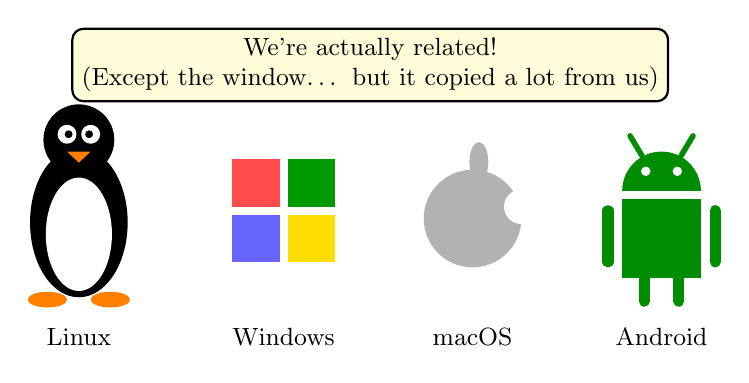
\begin{tikzpicture}[line width=0.8pt]
    % Penguin (Linux)
    \begin{scope}[shift={(0,0)}]
      \fill[black] (0,1.1) ellipse (0.62 and 0.95);
      \fill[white] (0,0.95) ellipse (0.42 and 0.72);
      \fill[black] (0,2.15) circle (0.45);
      \fill[white] (-0.15,2.22) circle (0.12) (0.15,2.22) circle (0.12);
      \fill[black] (-0.13,2.22) circle (0.05) (0.13,2.22) circle (0.05);
      \fill[orange] (-0.15,2.0) -- (0.15,2.0) -- (0,1.86) -- cycle;
      \fill[orange] (-0.4,0.12) ellipse (0.25 and 0.1) (0.4,0.12) ellipse (0.25 and 0.1);
      \node[font=\small] at (0,-0.35) {Linux};
    \end{scope}
    % Window (Windows)
    \begin{scope}[shift={(2.6,0.45)}]
      \fill[red!70]    (-0.65,0.85) rectangle (-0.05,1.45);
      \fill[green!60!black] (0.05,0.85) rectangle (0.65,1.45);
      \fill[blue!60]   (-0.65,0.15) rectangle (-0.05,0.75);
      \fill[yellow!80!orange] (0.05,0.15) rectangle (0.65,0.75);
      \node[font=\small] at (0,-0.8) {Windows};
    \end{scope}
    % Apple (macOS)
    \begin{scope}[shift={(5.0,0.25)}]
      \fill[gray!60] (0,0.9) circle (0.62);
      \fill[white] (0.62,1.05) circle (0.22);
      \fill[gray!60] (0.08,1.62) ellipse (0.12 and 0.25);
      \node[font=\small] at (0,-0.6) {macOS};
    \end{scope}
    % Robot (Android)
    \begin{scope}[shift={(7.4,0)}]
      \fill[green!55!black] (-0.5,0.4) rectangle (0.5,1.4);
      \fill[green!55!black] (-0.5,1.5) arc[start angle=180, end angle=0, radius=0.5];
      \fill[white] (-0.2,1.75) circle (0.06) (0.2,1.75) circle (0.06);
      \draw[green!55!black, line width=2pt, line cap=round] (-0.25,1.95) -- (-0.4,2.2) (0.25,1.95) -- (0.4,2.2);
      \draw[green!55!black, line width=4pt, line cap=round] (-0.68,0.6) -- (-0.68,1.25) (0.68,0.6) -- (0.68,1.25)
                                                          (-0.22,0.4) -- (-0.22,0.1) (0.22,0.4) -- (0.22,0.1);
      \node[font=\small] at (0,-0.35) {Android};
    \end{scope}
    \node[draw, rounded corners, fill=yellow!15, font=\small, align=center] at (3.7,3.1)
      {We're actually related!\\(Except the window\ldots{} but it copied a lot from us)};
  \end{tikzpicture}
  \caption{Today's ``Big Four''}
  \label{fig:four-os}
\end{figure}

\section{Why They Feel Different}

If the kernels all do much the same job, why does switching to another system feel so awkward? There are many reasons: the screens look different, the keyboard shortcuts are different, the built-in programs are different\ldots{} One of the most puzzling is \emph{how files are organized}.

\subsection{Windows: One Drive After Another}

On Windows, every hard disk (or every partition on a disk, or every USB stick) is a ``drive'', named by a letter: \texttt{C:}, \texttt{D:}, \texttt{E:}\ldots{} Each drive has its own tree of folders, and the trees have nothing to do with each other:
\begin{minted}[linenos=false]{text}
C:\
+-- Windows\          Windows itself
+-- Program Files\    installed software
`-- Users\
    `-- alex\         your files: Desktop, Documents, Downloads...
D:\
`-- work\
    `-- mypaper\      this book
\end{minted}
Paths are separated by backslashes, \texttt{\textbackslash}, as in \texttt{D:\textbackslash work\textbackslash mypaper}. Why start at C? Because \texttt{A:} and \texttt{B:} were kept for floppy disk drives. That was back in the days of DOS, but the rule has stuck around to this day. Upper and lower case don't matter either: \texttt{HELLO.C} and \texttt{hello.c} are the same file.

\subsection{Linux: Just One Tree}

Linux (and macOS, and Android) has no idea of ``drives''. The whole system is a single tree, and its root is called \texttt{/} (the root directory). Everything grows on this tree: hard disks, USB sticks, even the keyboard and the screen are just some folder or some file on the tree. Type \texttt{ls /} in a WSL terminal and you will see the folders under the root directory:
\begin{minted}[linenos=false]{text}
$ ls /
bin   boot  dev  etc  home  lib  media  mnt  opt  proc
root  run   sbin  srv  sys  tmp  usr  var
\end{minted}
Their names are all very short. They are abbreviations left over from the days of Unix (Table~\ref{tab:fhs}).

\begin{table}[htbp]
  \begin{lazywide}
  \caption{Common folders under the Linux root directory}
  \label{tab:fhs}
  \begin{tabular}{lL{3.8cm}L{6.0cm}}
    \toprule
    Folder & Short for & What's inside \\
    \midrule
    \texttt{/home} & home & Each user's ``home'': \texttt{/home/alex} is like \texttt{C:\textbackslash Users\textbackslash alex} on Windows \\
    \texttt{/bin}, \texttt{/usr/bin} & binary & Programs: \texttt{ls} and \texttt{gcc} live here \\
    \texttt{/lib}, \texttt{/usr/lib} & library & Libraries: \texttt{libc.so.6} is in \texttt{/usr/lib/x86\_64-linux-gnu/} \\
    \texttt{/usr/include} & include & Header files: \texttt{stdio.h} is here (Section~\ref{sec:stdio-h}) \\
    \texttt{/etc} & originally ``et cetera'' & The system's settings files \\
    \texttt{/tmp} & temporary & Temporary files, usually gone after a restart \\
    \texttt{/dev} & device & Devices: disks, terminals\ldots{} all show up here as files \\
    \texttt{/proc} & process & Information about running programs; the \texttt{/proc/self/maps} we read in Section~\ref{sec:layout} is here \\
    \texttt{/mnt}, \texttt{/media} & mount & Other disks and USB sticks are ``hung'' here \\
    \texttt{/root} & & The home of the superuser (the administrator). Don't mix it up with the root directory \texttt{/} \\
    \bottomrule
  \end{tabular}
  \end{lazywide}
\end{table}

So where did the other hard disk go? On Linux, you first have to ``mount''\lazynote{Mount}{To attach a disk (or USB stick) to a folder in the directory tree, so that you can reach it from there.} it on some folder in the tree before you can see it. That is exactly what WSL does: the Windows \texttt{C:} drive is mounted at \texttt{/mnt/c}, and the \texttt{D:} drive at \texttt{/mnt/d}. So this book lives in \texttt{D:\textbackslash work\textbackslash mypaper} on Windows and in \texttt{/mnt/d/work/mypaper} in WSL---the same folder, just called by two different names in two different systems. Linux paths are separated by forward slashes, \texttt{/}, and case matters: \texttt{Hello.c} and \texttt{hello.c} are two different files.

\begin{figure}[htbp]
  \centering
  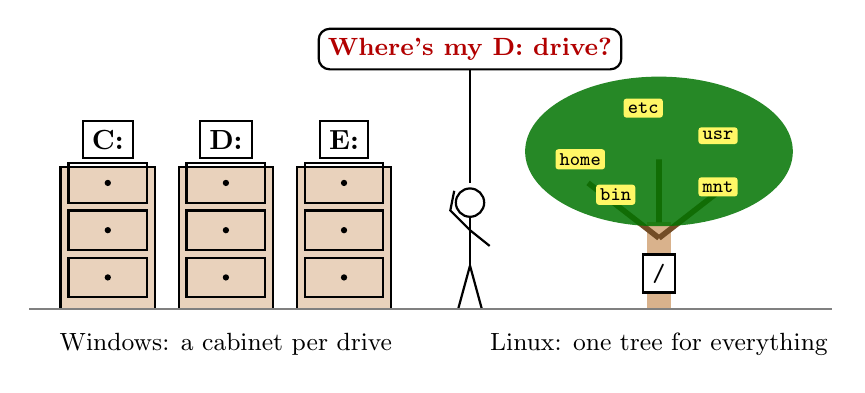
\begin{tikzpicture}[line width=0.8pt]
    % Left: a row of Windows cabinets
    \foreach \x/\l in {0/C, 1.5/D, 3.0/E} {
      \filldraw[fill=brown!35] (\x,0) rectangle +(1.2,1.8);
      \foreach \y in {0.15,0.75,1.35} \draw (\x+0.1,\y) rectangle +(1.0,0.5);
      \foreach \y in {0.4,1.0,1.6} \fill (\x+0.6,\y) circle (0.04);
      \node[draw, fill=white, font=\bfseries] at (\x+0.6,2.15) {\l:};
    }
    \node[font=\small] at (2.1,-0.45) {Windows: a cabinet per drive};
    % Right: the Linux tree
    \begin{scope}[shift={(7.6,0)}]
      \fill[brown!60] (-0.15,0) rectangle (0.15,1.1);
      \draw[brown!60!black, line width=2pt] (0,0.9) -- (-0.9,1.6) (0,0.9) -- (0.9,1.6) (0,1.1) -- (0,1.9);
      \fill[green!45!black, opacity=0.85] (0,2.0) ellipse (1.7 and 0.95);
      \node[draw, fill=white, font=\ttfamily\small] at (0,0.45) {/};
      \foreach \x/\y/\t in {-1.0/1.9/home, -0.2/2.55/etc, 0.75/2.2/usr, -0.55/1.45/bin, 0.75/1.55/mnt} {
        \node[fill=yellow!60, font=\ttfamily\scriptsize, inner sep=1.5pt, rounded corners=1pt] at (\x,\y) {\t};
      }
      \node[font=\small] at (0,-0.45) {Linux: one tree for everything};
    \end{scope}
    % A puzzled little person walking from the cabinets to the tree
    \draw (5.2,1.35) circle (0.18);
    \draw (5.2,1.17) -- (5.2,0.55);
    \draw (5.2,0.55) -- (5.05,0) (5.2,0.55) -- (5.35,0);
    \draw (5.2,1.0) -- (4.95,1.25) -- (5.0,1.5);
    \draw (5.2,1.0) -- (5.45,0.8);
    \node[draw, rounded corners, fill=white, text=red!70!black, font=\small\bfseries] (q) at (5.2,3.3) {Where's my D: drive?};
    \draw (q.south) -- (5.2,1.6);
    \draw[gray, line width=1pt] (-0.4,0) -- (9.8,0);
  \end{tikzpicture}
  \caption{Cabinets and a tree}
  \label{fig:drives-tree}
\end{figure}

Both ways work, and neither is right or wrong. If it feels strange at first, that's only because you're not used to it. You don't have to figure it all out at once. Just accept that ``this is how they organize things'', and you'll get used to it as you go.

\section{Why GCC, Even on \texorpdfstring{\NoCaseChange{Windows}}{Windows}?}

This book uses \texttt{gcc} to compile programs from beginning to end. Even the Windows programs are compiled with the MinGW version of gcc (Section~\ref{sec:win32}). Why not use Microsoft's own compiler?

The simplest reason: \textbf{it's free}. It is also free software\lazynote{Free software}{Software that you are free to use, study, change and share. Its source code is public.}: anyone may download it, use it, and even change its source code. GCC was released by the GNU Project in 1987. At first it was called the ``GNU C Compiler''; later it learned more and more languages and was renamed the ``GNU Compiler Collection''. Today it can produce code for dozens of CPUs: x86, ARM, RISC-V\ldots{} And if you ever build your own CPU, the compiler you use for its programs will most likely be gcc, too.

Of course, gcc is not the only good compiler. Microsoft's Visual Studio (with its MSVC compiler) has a free Community edition and is very handy for writing graphical programs on Windows. Apple's Xcode, and Clang, which is also popular on Linux, are free as well. For learning C, any of them will do. This book picks gcc because it works on both Linux and Windows (through WSL or MinGW), with the same commands everywhere.

\section{The Terminal and the Graphical Interface}

An operating system has two faces. One is the \emph{terminal}\lazynote{Terminal}{A window where you type commands and see text results. The \texttt{bash} running inside it is called a shell.} (the command line), with its plain text on a black background. The other is the \emph{graphical user interface} (GUI), with windows, icons and a mouse. Many people think the terminal is an ``old relic'' and the GUI is ``advanced''---or the other way round, that only people who type commands are ``real experts''. In fact neither is better than the other; they are just good at different things (Figure~\ref{fig:cli-gui}).

\begin{figure}[htbp]
  \centering
  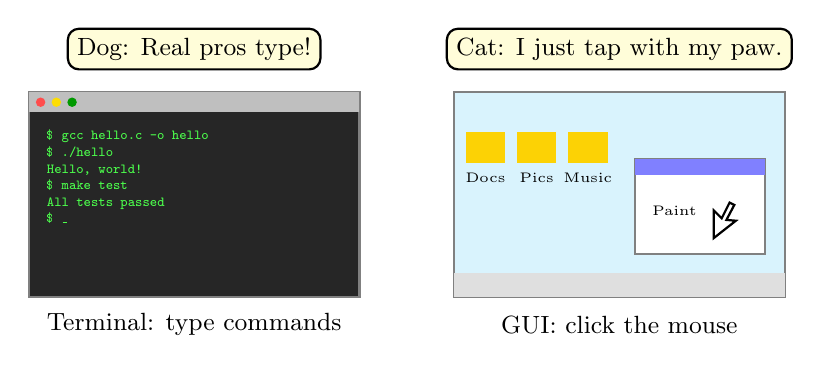
\begin{tikzpicture}[line width=0.8pt]
    % Terminal
    \filldraw[fill=black!85, draw=gray] (0,0) rectangle (4.2,2.6);
    \fill[gray!50] (0,2.35) rectangle (4.2,2.6);
    \foreach \x/\c in {0.15/red!70, 0.35/yellow!80!orange, 0.55/green!60!black} \fill[\c] (\x,2.475) circle (0.06);
    \node[anchor=north west, align=left, font=\ttfamily\tiny, text=green!70] at (0.1,2.25)
      {\$ gcc hello.c -o hello\\\$ ./hello\\Hello, world!\\\$ make test\\All tests passed\\\$ \_};
    \node[font=\small] at (2.1,-0.35) {Terminal: type commands};
    % GUI
    \begin{scope}[shift={(5.4,0)}]
      \filldraw[fill=cyan!15, draw=gray] (0,0) rectangle (4.2,2.6);
      \fill[gray!25] (0,0) rectangle (4.2,0.3);
      \foreach \x/\y/\t in {0.4/1.9/Docs, 1.05/1.9/Pics, 1.7/1.9/Music} {
        \fill[yellow!70!orange] (\x-0.25,\y-0.2) rectangle (\x+0.25,\y+0.2);
        \node[font=\tiny] at (\x,\y-0.38) {\t};
      }
      \filldraw[fill=white, draw=gray] (2.3,0.55) rectangle (3.95,1.75);
      \fill[blue!50] (2.3,1.55) rectangle (3.95,1.75);
      \node[font=\tiny] at (2.8,1.1) {Paint};
      \draw[fill=white] (3.3,0.75) -- (3.3,1.1) -- (3.4,1.0) -- (3.5,1.2) -- (3.56,1.17) -- (3.46,0.98) -- (3.58,0.97) -- cycle;
      \node[font=\small] at (2.1,-0.35) {GUI: click the mouse};
    \end{scope}
    % The dog and the cat
    \node[draw, rounded corners, fill=yellow!15, font=\small] at (2.1,3.15) {Dog: Real pros type!};
    \node[draw, rounded corners, fill=yellow!15, font=\small] at (7.5,3.15) {Cat: I just tap with my paw.};
  \end{tikzpicture}
  \caption{The terminal and the GUI: they do different jobs, and neither is better than the other}
  \label{fig:cli-gui}
\end{figure}

\paragraph{What the terminal is better at:}
\begin{itemize}
  \item \textbf{Repetition and batches.} Renaming a hundred photos takes one command in the terminal, but a hundred rounds of clicking with the mouse. The \texttt{make test} in this book runs dozens of programs in one go.
  \item \textbf{Precision and repeatability.} Commands can be saved in a file and run again exactly as before, with exactly the same results. Every piece of program output in this book was produced automatically this way.
  \item \textbf{Remote control.} Servers often have no screen at all. Administrators connect to them over the network and do everything in a terminal.
  \item \textbf{Programming.} Compiling, debugging, watching system calls (\texttt{strace})\ldots{} most of a programmer's tools are used in the terminal.
\end{itemize}

\paragraph{What the GUI is better at:}
\begin{itemize}
  \item \textbf{Looking and drawing.} Viewing photos, watching videos, editing pictures, drawing---these are nearly impossible without a screen and a mouse.
  \item \textbf{Exploring.} When you use a program for the first time, its menus and buttons show you what it can do. You don't have to learn any commands first.
  \item \textbf{Everyday use.} Browsing the web, chatting, writing documents, playing games---most people spend most of their time in a GUI.
\end{itemize}

In fact, this book was written using both faces: drafts were written in Vim and compiled with \texttt{latexmk} in the terminal, and the layout was checked in a graphical PDF viewer. And whether it's the terminal or the GUI, both are just ordinary programs: \texttt{bash} in the terminal and \texttt{explorer.exe}, the Windows desktop, both end up asking the kernel for help through system calls. To the kernel, there is no difference between them at all.

\section{Summary}

\begin{itemize}
  \item Today's Windows, Linux, macOS and Android are all modern operating systems, and they do much the same job. They come from two ancestors, Unix and DOS: macOS comes from BSD, Android uses the Linux kernel, and today's Windows uses the NT kernel.
  \item One reason they feel ``different'' is the way files are organized: Windows uses drives such as \texttt{C:} and \texttt{D:}; Linux has just one tree with \texttt{/} as its root, and other disks are mounted onto the tree.
  \item GCC is free of charge and free software. It compiles programs for many kinds of CPU, and it works on both Linux and Windows.
  \item The terminal and the GUI are the two faces of an operating system. Each is good at different things; neither is better.
  \item You don't need to understand all of this at once. Learning operating systems takes years; for now, ``oh, so that's how it is'' is enough.
\end{itemize}
